\chapter{Evaluation and Results}\label{ch:evaluation}

%% ===================================================================
\section{RQ1: Description Quality Across Models and Languages}\label{sec:rq1-results}
%% ===================================================================

We evaluate 13 VLMs on 120 scientific figures spanning four languages using our Atomic MQM framework with two LLM judges (GPT-4o, Mistral Large~3).
This section reports the model leaderboard (\S\ref{sec:rq1-leaderboard}), validates the judge framework against human annotations (\S\ref{sec:rq1-human}), and characterises the dominant error patterns (\S\ref{sec:rq1-errors}).

\subsection{Model Leaderboard}\label{sec:rq1-leaderboard}

Table~\ref{tab:leaderboard} ranks all 13 models by normalised Atomic MQM (0--100$\uparrow$), reporting per-judge scores with 95\% bootstrap CIs ($n{=}10\text{k}$ resamples), per-language breakdowns, mean error counts, and hallucination rates.

\begin{table}[t]
\centering
\caption{\textbf{RQ1 core results.}
  \textbf{(a)}~Model leaderboard ranked by judge-averaged Atomic MQM (0--100\,$\uparrow$). G = GPT-4o judge, M = Mistral Large~3 judge, Avg = mean of both. Language columns (EN = English, BG = Bulgarian, CN = Chinese, DE = German) show judge-averaged scores. E = mean MQM errors/fig ($\downarrow$). H = mean fabrications/fig ($\downarrow$), a subset of E. CI shown as $\pm$ half-width (95\% bootstrap, $10\text{k}$ resamples). Significance vs.\ next rank (paired bootstrap): $^{***}\!p{<}.001$, $^{*}\!p{<}.05$; unmarked = not significant. \textbf{Bold} = best, \underline{underline} = 2nd best per column.
  \textbf{(b)}~Error sub-type distribution across 26\,364 errors (both judges, all models). M\% = proportion assigned Major severity (examples in Table~\ref{tab:error-examples}).
  \textbf{(c)}~Human--judge validation on 30 English figures (3 annotators, 159 annotations). Bias = judge $-$ human (negative = judge harsher). Segment-level correlations over $n{=}120$ (figure, model) pairs; system-level over 4 model averages. IAA = inter-annotator agreement on 39 double-annotated pairs. ICC = intraclass correlation coefficient.
  \textbf{(d)}~MQM by chart type (judge-averaged, all models). $\bar{a}$ = mean atoms per figure. $\Delta_{\text{cap}}$ = MQM gain from capping at one error per atom, isolating the normalisation artefact.
}\label{tab:leaderboard}\label{tab:errors-charts}\label{tab:human-judge}
\vspace{-2pt}
\scriptsize
\setlength{\tabcolsep}{2pt}
%%% Row 1: (a) Leaderboard + (b) Error distribution
\begin{minipage}[t]{0.66\textwidth}
\centering
\textbf{(a) Model leaderboard}\\[2pt]
\begin{tabular}{@{}r@{\;}l@{\;\;}r@{\,}l@{\;\;}r@{\,}l@{\;\;}r@{\;\;}rrrr@{\;\;}r@{\;}r@{}}
\toprule
 & & \multicolumn{2}{c}{\textbf{G}} & \multicolumn{2}{c}{\textbf{M}} & \textbf{Avg} & \textbf{EN} & \textbf{BG} & \textbf{CN} & \textbf{DE} & \textbf{E} & \textbf{H} \\
\midrule
1$^{***}$ & GPT-5.2              & \textbf{72.0} & {\tiny$_{\pm3}$} & \textbf{79.0} & {\tiny$_{\pm2}$} & \textbf{75.5} & \textbf{75.5} & \textbf{72.2} & \textbf{76.1} & \textbf{81.1} & \textbf{7.2} & \textbf{.14} \\
2$^{*}$   & Gemini 3.1P          & \underline{70.4} & {\tiny$_{\pm3}$} & \underline{74.9} & {\tiny$_{\pm3}$} & \underline{72.7} & \underline{69.0} & \underline{72.0} & \underline{75.0} & 77.2 & 7.8 & .25 \\
3         & Qwen 235B            & 67.2 & {\tiny$_{\pm3}$} & 74.4 & {\tiny$_{\pm3}$} & 70.8 & 68.5 & 68.4 & 69.7 & 77.2 & 7.9 & .25 \\
4         & Qwen 32B             & 68.7 & {\tiny$_{\pm3}$} & 72.1 & {\tiny$_{\pm3}$} & 70.4 & 68.9 & 65.6 & 71.9 & 78.2 & 8.0 & .31 \\
5         & Claude 4.6           & 66.2 & {\tiny$_{\pm4}$} & 71.0 & {\tiny$_{\pm4}$} & 68.6 & 64.4 & 64.1 & 70.5 & \underline{79.6} & 7.7 & \underline{.09} \\
6         & LLaMA Mav.           & 65.0 & {\tiny$_{\pm4}$} & 70.7 & {\tiny$_{\pm4}$} & 67.8 & 65.3 & 65.7 & 68.2 & 73.1 & 8.6 & .20 \\
7         & LLaMA Scout          & 64.6 & {\tiny$_{\pm4}$} & 69.6 & {\tiny$_{\pm4}$} & 67.1 & 65.0 & 65.2 & 68.8 & 73.1 & 8.6 & .23 \\
8         & Qwen 30B             & 64.3 & {\tiny$_{\pm4}$} & 69.3 & {\tiny$_{\pm4}$} & 66.8 & 64.3 & 63.0 & 68.0 & 74.8 & 8.5 & .25 \\
9$^{***}$ & Qwen 8B              & 63.8 & {\tiny$_{\pm4}$} & 69.6 & {\tiny$_{\pm4}$} & 66.7 & 64.2 & 60.9 & 70.8 & 74.8 & 8.5 & .34 \\
\cmidrule(lr){1-13}
10        & Gemma 27B            & 57.1 & {\tiny$_{\pm4}$} & 60.5 & {\tiny$_{\pm4}$} & 58.8 & 53.3 & 60.5 & 60.0 & 64.5 & 9.9 & .35 \\
11$^{*}$  & Phi-4                & 57.8 & {\tiny$_{\pm6}$} & 57.0 & {\tiny$_{\pm6}$} & 57.4 & 57.2 & 51.3 & 56.2 & 65.7 & 10.9 & .50 \\
12$^{***}$& Gemma 12B            & 54.3 & {\tiny$_{\pm4}$} & 52.8 & {\tiny$_{\pm4}$} & 53.6 & 52.4 & 49.0 & 52.4 & 61.3 & 10.8 & .47 \\
13        & Gemma 4B             & 50.5 & {\tiny$_{\pm4}$} & 46.5 & {\tiny$_{\pm4}$} & 48.5 & 44.3 & 46.1 & 48.7 & 58.1 & 11.8 & .65 \\
\bottomrule
\end{tabular}
\end{minipage}%
\hfill
\begin{minipage}[t]{0.32\textwidth}
\centering
\textbf{(b) Error distribution}\\[2pt]
\begin{tabular}{@{}lrrr@{}}
\toprule
\textbf{Sub-type} & \textbf{n} & \textbf{\%} & \textbf{M\%} \\
\midrule
\multicolumn{4}{@{}l}{\textit{Accuracy (53.9\%)}} \\
\;\; Num.\ Value      & 8057 & 30.6 & 77 \\
\;\; Vis.\ Attrib.    & 4289 & 16.3 & 71 \\
\;\; Struct.\ Desc.   &  854 &  3.2 & 68 \\
\;\; Axis/Legend      &  853 &  3.2 & 65 \\
\midrule
\multicolumn{4}{@{}l}{\textit{Completeness (41.4\%)}} \\
\;\; Miss.\ Visual    & 6020 & 22.8 & 46 \\
\;\; Miss.\ Purpose   & 1666 &  6.3 & 61 \\
\;\; Miss.\ Axis      & 1128 &  4.3 & 54 \\
\;\; Hallucination    &  947 &  3.6 & 92 \\
\;\; Unwant.\ Interp. &  482 &  1.8 & 38 \\
\midrule
\multicolumn{4}{@{}l}{\textit{Clarity (4.7\%)}} \\
\;\; Ambig./Verbose   & 1213 &  4.6 &  3 \\
\;\; Poor Struct.     &  173 &  0.7 &  2 \\
\bottomrule
\end{tabular}
\end{minipage}

\vspace{6pt}
%%% Row 2: (c) Human-judge validation + (d) Chart-type MQM
\begin{minipage}[t]{0.62\textwidth}
\centering
\textbf{(c) Human--judge validation}\\[2pt]
\begin{tabular}{@{}l rrr rr rr@{}}
\toprule
 & \multicolumn{3}{c}{\textbf{Human}} & \multicolumn{2}{c}{\textbf{GPT-4o}} & \multicolumn{2}{c}{\textbf{Mistral}} \\
\cmidrule(lr){2-4}\cmidrule(lr){5-6}\cmidrule(lr){7-8}
\textbf{Model} & MQM & E/fig & $n$ & MQM & bias & MQM & bias \\
\midrule
GPT-5.2        & \textbf{97.0} & \textbf{0.8} & 40 & 71.6 & $-$25.6 & 79.3 & $-$17.9 \\
Qwen 30B       & 76.2 & 4.1 & 40 & 63.4 & $-$13.0 & 65.2 & $-$11.2 \\
Qwen 8B        & 76.2 & 5.3 & 39 & 62.2 & $-$12.0 & 66.2 & $-$8.0 \\
Gemma 27B      & 59.9 & 9.0 & 40 & 49.6 & $-$9.4 & 56.9 & $-$2.2 \\
\midrule
\multicolumn{8}{@{}l}{\textit{Corr.\ (seg\,/\,sys):}\; $\rho$\; .58/.95 (G)\; \textbf{.65/.95} (M)\; .69/.97 (G$\leftrightarrow$M)} \\
\multicolumn{8}{@{}l}{\textit{IAA:}\; ICC=.91\; $\rho$=.85\; $r$=.92\; mean $\Delta$=7.6\,pts\; (69\% $\leq$10)} \\
\multicolumn{8}{@{}l}{\textit{Severity:}\; G 78\% Major\; M 47\% Major\; \textit{Bias:}\; G $-$15.0\; M $-$9.8} \\
\bottomrule
\end{tabular}
\end{minipage}%
\hfill
\begin{minipage}[t]{0.36\textwidth}
\centering
\textbf{(d) Chart-type difficulty}\\[2pt]
\begin{tabular}{@{}lrr rr r@{}}
\toprule
\textbf{Type} & $n$ & $\bar{a}$ & \textbf{MQM} & \textbf{E/fig} & $\Delta_{\text{cap}}$ \\
\midrule
Line   & 43 & 19.2 & 70.5 &  8.1 & +2.3 \\
Bar    & 43 & 18.7 & 69.3 &  8.5 & +3.8 \\
Pie    & 34 & 10.8 & 54.1 & 10.2 & \textbf{+11.0} \\
\midrule
\multicolumn{6}{@{}l}{\textit{Hallucination by tier}} \\
\midrule
\multicolumn{3}{@{}l}{T1 (GPT, Gem.)} & \multicolumn{3}{r}{.14--.25} \\
\multicolumn{3}{@{}l}{T2 (Qw, LL, Cl)} & \multicolumn{3}{r}{.09--.34} \\
\multicolumn{3}{@{}l}{T3 (Gma, Phi)} & \multicolumn{3}{r}{.35--.65} \\
\bottomrule
\end{tabular}
\end{minipage}
\end{table}

Three statistically distinct tiers emerge (paired bootstrap, $p{<}.05$).
\textbf{Tier~1}~(75--73): GPT-5.2 and Gemini, separated from all others.
\textbf{Tier~2}~(71--67): Qwen-235B through Qwen-8B form an indistinguishable cluster; Claude and both LLaMA-4 variants fall here too.
\textbf{Tier~3}~(59--49): Gemma and Phi, each step significantly worse.
The proprietary--open gap is narrow at the top (GPT-5.2 leads Qwen-235B by 4.7) but widens sharply below rank~9.

German yields the highest per-language scores (mean~72.5) across all models, while Bulgarian trails (62.4).
However, our controlled cross-lingual experiment (\S\ref{sec:rq1-ablations}) reverses this ranking when the same figures are evaluated in all four languages, revealing dataset composition rather than language capability as the primary driver.

Within model families, scaling shows diminishing returns. Qwen 235B $\approx$ 32B ($\Delta{=}0.4$, $p{=}.34$) but both significantly exceed 30B/8B, while Gemma shows steeper gains ($\Delta{=}5$ per step, all $p{<}.001$).
Figure~\ref{fig:heatmap} provides a dense visual summary across all models and languages.

\begin{figure}[t]
  \centering
  \begin{subfigure}[t]{0.52\textwidth}
    \centering
    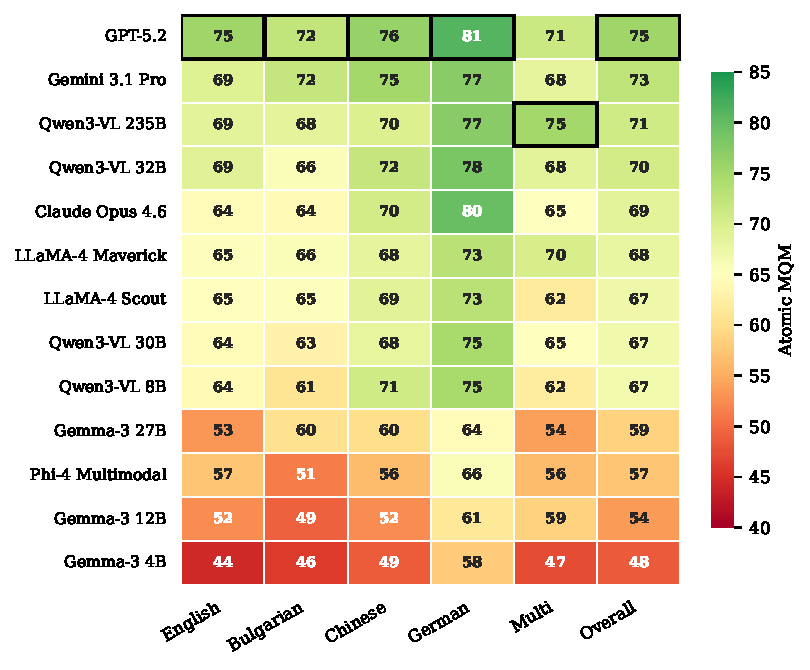
\includegraphics[width=\textwidth]{figures/rq1/heatmap_model_lang.pdf}
    \caption{Model$\times$Language MQM (judge-averaged). Black box = column best.}
    \label{fig:heatmap}
  \end{subfigure}%
  \hfill
  \begin{subfigure}[t]{0.46\textwidth}
    \centering
    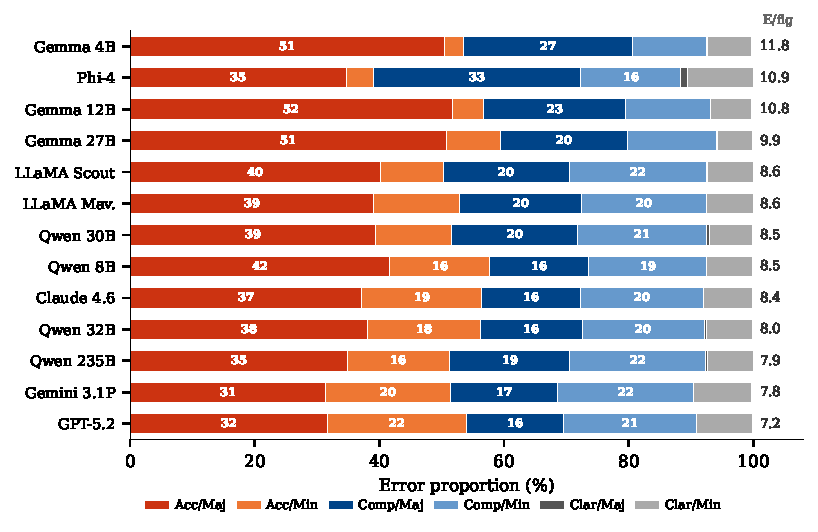
\includegraphics[width=\textwidth]{figures/rq1/error_stacked.pdf}
    \caption{Error composition (100\% stacked). Right = errors/fig.}
    \label{fig:error-stacked}
  \end{subfigure}
  \caption{\textbf{(a)} Per-language performance heatmap. German leads in uncontrolled comparison; the controlled study (\S\ref{sec:rq1-ablations}) reverses this. \textbf{(b)} Error-type proportions per model. Accuracy/Major (red) dominates; weaker models show larger Completeness/Major (blue) shares.}
  \label{fig:heatmap-errors}
\end{figure}

%% -------------------------------------------------------------------
\subsection{Judge Validation Against Human Annotation}\label{sec:rq1-human}
%% -------------------------------------------------------------------

Three annotators evaluated four models on 30~English figures (159~annotations, 39~double-annotated).
Table~\ref{tab:human-judge}(c) reports the results.

The central finding is a \emph{ranking--scoring dissociation}: all evaluators agree near-perfectly on model ordering (system-level $\rho{\geq}.95$, judge--judge $\rho{=}.97$), yet absolute scores diverge by 10--25 points.
Both judges are systematically harsher than humans, with the bias largest for the best model (GPT-5.2: $-$25.6 from GPT-4o) and smallest for the weakest (Gemma-27B: $-$2.2 from Mistral).
This asymmetric compression indicates that judges are more sensitive to minor imprecisions in otherwise strong descriptions.

The two judges diverge primarily in severity assignment: GPT-4o marks 78\% of errors as Major vs.\ Mistral's 47\%, directly inflating GPT-4o's penalty weights.
Averaging two judges with complementary severity profiles stabilises the evaluation.
Human inter-annotator agreement is excellent (ICC\,=\,.91), confirming that the Atomic MQM rubric yields reproducible human judgements.
Figure~\ref{fig:scatter} visualises this relationship.

\begin{figure}[!ht]
  \centering
  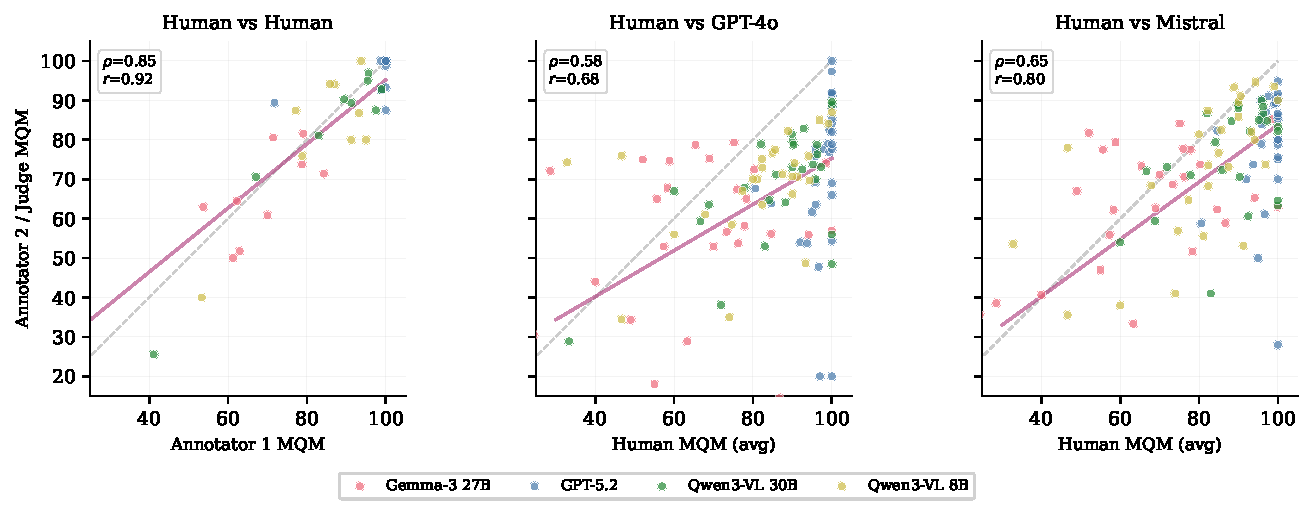
\includegraphics[width=\textwidth]{figures/rq1/scatter_human_judge.pdf}
  \vspace{-8pt}
  \caption{\textbf{Evaluator agreement.} Left: inter-annotator (39 pairs, $\rho{=}.85$). Centre/Right: human vs.\ LLM judge (120 pairs). Dashed = identity; solid = regression. Below diagonal = judge harsher.}
  \label{fig:scatter}
\end{figure}

%% -------------------------------------------------------------------
\subsection{Error Analysis}\label{sec:rq1-errors}
%% -------------------------------------------------------------------

Across 2\,966 evaluations, the judges flagged 26\,364 errors (8.9/fig).
Table~\ref{tab:errors-charts}(b) summarises the aggregate error distribution; the full per-model per-judge breakdown is in Appendix Table~\ref{tab:error-profile-full}.
Accuracy errors dominate, with \emph{Incorrect Numerical Value} alone at 30.6\%, making it the primary bottleneck across all models.
Hallucinated Content, though only 3.6\% of errors, carries 92\% Major severity and correlates inversely with model capacity.
Pie charts score 15--25 points below line/bar charts; the $\Delta_{\text{cap}}$ column in Table~\ref{tab:errors-charts}(d) confirms that ${\sim}11$ of those points stem from multi-error atoms rather than genuine difficulty.
Colour-synonym false positives remain a systematic judge limitation (${\sim}5\%$ penalty on English vs.\ ${\sim}2\%$ on Chinese).
Figure~\ref{fig:error-stacked} shows the per-model error composition.

%% -------------------------------------------------------------------
\subsection{Ablation Studies}\label{sec:rq1-ablations}
%% -------------------------------------------------------------------

\paragraph{Cross-lingual controlled comparison.}
We evaluate 13 parallel figures (same figure, all four languages) with language-specific atom checklists on five models spanning the performance range.
The controlled results \emph{reverse} the uncontrolled language ranking. English scores highest for all models (GPT-5.2 at EN~66.2 $>$ CN~60.8 $>$ BG~56.4 $>$ DE~55.3), confirming that the German advantage in Table~\ref{tab:leaderboard} is a dataset composition artefact.
Chinese is the most resilient non-English language (EN--CN gap 4--17\%), while smaller models degrade disproportionately (Gemma-4B: 42\% EN--DE gap vs.\ Claude's 2\%).

\paragraph{Prompt language (C1 vs C2).}
We tested whether switching the instruction language from native to English (while keeping output in the native language) affects description quality.
Raw MQM scores suggest a ${\sim}10$-point drop under C2 (Appendix Table~\ref{tab:app-ablation-prompt}), but independent manual comparison of the C1 and C2 descriptions across all three non-English languages found no substantive quality difference: the descriptions contain the same values, the same structural observations, and the same error patterns.
The MQM gap is attributable to judge severity inconsistency across separate evaluation calls (the judge assigns different severity to identical errors when scoring different descriptions), reinforcing the segment-level unreliability documented in \S\ref{sec:rq1-human}.
GPT-5.2 is instruction-language robust for non-English figure description.

\paragraph{Chain-of-thought.}
CCoT prompting~\citep{mitra2024ccot} helps weaker models (Phi-4: $+$9pp, LLaMA Maverick: $+$6pp) but \emph{hurts} stronger ones (GPT-5.2: $-$15pp, Qwen-8B: $-$13pp), suggesting that explicit reasoning can interfere with well-calibrated models.
Full per-model results and methodological notes are in Appendix Table~\ref{tab:cot-ablation-full}.

%% ===================================================================
\section{RQ2: Degradation Under Adversarial Transforms}\label{sec:rq2-results}
%% ===================================================================

We apply five image transforms and two page-context conditions to 45~figures and re-evaluate all 13~models with both judges.
The five transforms simulate realistic quality degradation: JPEG compression (quality=15), Gaussian noise ($\sigma{=}30$), aspect-ratio distortion (1.2$\times$ horizontal stretch), low contrast (50\% reduction), and 30$^\circ$ rotation.
Two additional conditions test page context: \emph{original-in-paper} (the figure as it appears on the PDF page, with surrounding text) and \emph{blurred-in-paper} (same but with the figure region blurred), probing whether models extract contextual cues from surrounding paper content.

Table~\ref{tab:degradation} reports MQM scores and deltas from the clean original for each model and transform.
Figure~\ref{fig:degradation-slope} visualises the degradation trajectories.

\begin{table}[!ht]
\centering
\scriptsize
\setlength{\tabcolsep}{2.5pt}
\caption{\textbf{RQ2: Transform degradation} (45 figures, judge-averaged MQM).
  Orig = clean extracted figure. All other columns show $\Delta$ from Original.
  \emph{Page context}: InP = figure on its PDF page; BlurP = same page with figure blurred (diagnostic, tests whether models extract cues from surrounding text).
  \emph{Image transforms}: JPEG--Rotat.
  $|\bar{\Delta}|$ = mean absolute delta across the five image transforms only ($\downarrow$ = more robust).
  Sorted by $|\bar{\Delta}|$ ($\uparrow$). \textbf{Bold} = most robust; \underline{underline} = 2nd.
}\label{tab:degradation}
\begin{tabular}{@{}l r rr rrrrr r@{}}
\toprule
 & & \multicolumn{2}{c}{\textit{Page context}} & \multicolumn{5}{c}{\textit{Image transforms}} & \\
\cmidrule(lr){3-4}\cmidrule(lr){5-9}
 & \textbf{Orig} & \textbf{InP} & \cellcolor{gray!8}\textbf{BlurP} & \textbf{JPEG} & \textbf{Noise} & \textbf{Aspct} & \textbf{LoCon} & \textbf{Rotat} & $|\bar{\Delta}|$ \\
\midrule
Qwen 235B      & 71.1 & $-$8.7 & \cellcolor{gray!8}$-$14.7 & $-$1.0 & $-$0.2 & $-$0.5 & +1.3 & $-$5.0 & \textbf{1.6} \\
Gemini 3.1P    & 71.6 & \textbf{+5.7} & \cellcolor{gray!8}$-$6.2 & $-$0.1 & $-$1.3 & $-$0.1 & $-$3.1 & $-$4.8 & \underline{1.9} \\
Claude 4.6     & 66.1 & $-$4.1 & \cellcolor{gray!8}$-$8.0 & +1.1 & +1.4 & +1.6 & +2.2 & $-$3.2 & \underline{1.9} \\
GPT-5.2        & 69.7 & $-$1.7 & \cellcolor{gray!8}$-$8.3 & +2.5 & +1.2 & +3.1 & +0.3 & $-$2.7 & 2.0 \\
Phi-4          & 60.1 & +18.9 & \cellcolor{gray!8}+9.4 & +1.6 & $-$2.4 & $-$0.7 & +4.5 & +1.9 & 2.2 \\
LLaMA Mav.     & 68.9 & $-$5.0 & \cellcolor{gray!8}$-$9.0 & +1.7 & $-$0.3 & $-$0.0 & $-$0.7 & $-$9.0 & 2.4 \\
Gemma 4B       & 53.0 & $-$10.7 & \cellcolor{gray!8}$-$3.2 & $-$3.8 & $-$5.9 & $-$1.6 & $-$2.0 & +1.2 & 2.9 \\
Qwen 8B        & 66.7 & $-$2.7 & \cellcolor{gray!8}$-$10.4 & +4.9 & +1.4 & +7.1 & $-$4.1 & +1.6 & 3.8 \\
Qwen 30B       & 69.1 & $-$13.1 & \cellcolor{gray!8}$-$19.2 & +1.3 & +1.3 & +2.0 & +9.5 & $-$6.2 & 4.1 \\
Gemma 12B      & 54.5 & $-$5.0 & \cellcolor{gray!8}$-$3.1 & $-$4.2 & $-$0.4 & +8.2 & $-$4.1 & $-$10.7 & 5.5 \\
Gemma 27B      & 61.2 & $-$14.7 & \cellcolor{gray!8}$-$15.8 & $-$4.4 & +0.9 & $-$12.0 & $-$3.0 & $-$9.2 & 5.9 \\
Qwen 32B       & 70.1 & $-$4.6 & \cellcolor{gray!8}$-$21.2 & +8.3 & +3.7 & $-$6.7 & $-$6.4 & $-$5.8 & 6.2 \\
LLaMA Scout    & 71.0 & $-$16.9 & \cellcolor{gray!8}$-$18.6 & $-$5.4 & $-$5.2 & $-$0.4 & $-$10.6 & $-$9.6 & 6.2 \\
\bottomrule
\end{tabular}
\end{table}

\begin{figure}[t]
  \centering
  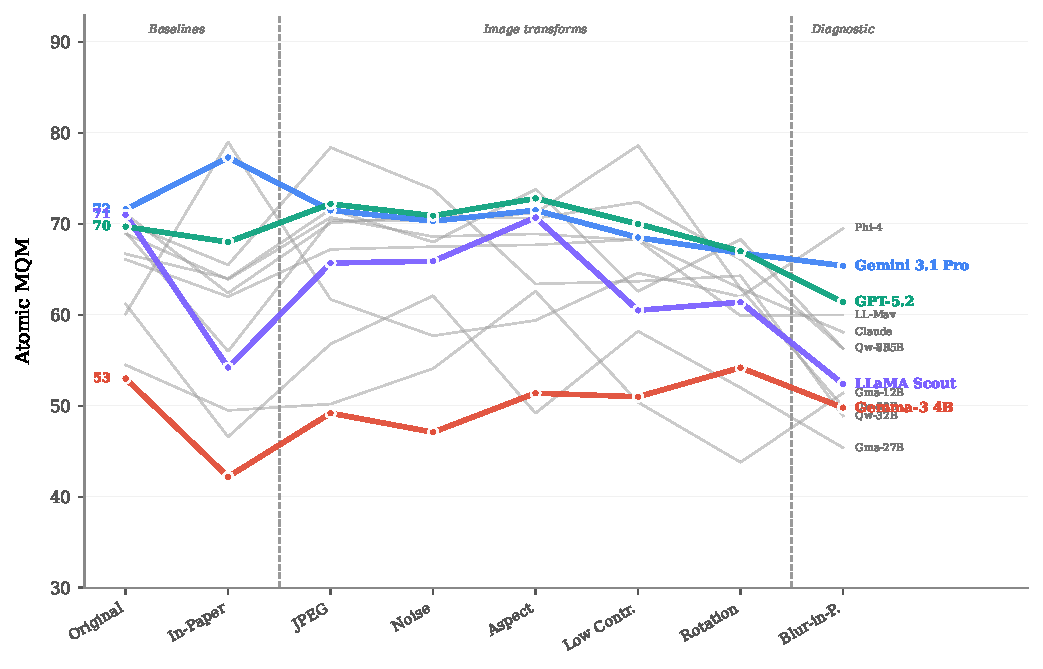
\includegraphics[width=0.85\textwidth]{figures/rq2/degradation_slope.pdf}
  \caption{\textbf{Degradation slope chart.} Each line traces a model's MQM across transforms (left to right = increasing severity). Solid blue = Tier~1 (proprietary), dashed green = Tier~2 (mid-range open), dotted pink = Tier~3 (small). Shaded zones separate baselines, image transforms, and the severe blur-in-paper diagnostic. Tier~1 models maintain the flattest profiles.}
  \label{fig:degradation-slope}
\end{figure}

Three findings emerge from the degradation analysis.

First, \textbf{rotation and low contrast cause the largest real-world degradation}.
Rotation ($\Delta{=}{-}4.7$ mean across models) and low contrast ($\Delta{=}{-}1.2$) are the most damaging image transforms, while JPEG compression ($\Delta{=}{+}0.2$) and noise ($\Delta{=}{-}0.4$) have negligible mean effect.
This suggests that VLMs are reasonably robust to pixel-level corruption but struggle when spatial layout is disrupted (rotation) or visual contrast is reduced.

Second, \textbf{robustness correlates with but is not determined by baseline quality}.
Qwen3-VL 235B ($|\bar{\Delta}|{=}1.6$), Gemini 3.1 Pro ($|\bar{\Delta}|{=}1.9$), and Claude Opus ($|\bar{\Delta}|{=}1.9$) are the most robust, maintaining stable scores across all transforms.
However, some mid-tier models show surprising volatility: Qwen-32B swings from $+$8.3 (JPEG) to $-$6.7 (aspect ratio), and LLaMA Scout drops $-$10.6 under low contrast.
This inconsistency suggests that robustness is a distinct capability from baseline accuracy.

Third, \textbf{the page-context conditions reveal divergent model strategies}.
Gemini scores \emph{higher} when the figure is shown in its paper context ($+$5.7), suggesting it extracts useful cues from surrounding text.
Conversely, LLaMA Scout ($-$16.9) and Gemma-27B ($-$14.7) degrade substantially in the in-paper condition, indicating that page context introduces noise for these models.
Phi-4 shows the most extreme context sensitivity ($+$18.9 in-paper), likely because its multimodal architecture was trained on document-level inputs.
The blurred-in-paper condition (not shown in the robustness metric) serves as a control: when the figure is unreadable but paper text remains, models that rely on context will still produce descriptions, while models that attend primarily to the figure will correctly report limited information.

%% ===================================================================
\section{RQ3: Comprehension Beyond Description}\label{sec:rq3-results}
%% ===================================================================

RQ3 moves beyond surface-level description to test whether models can answer questions \emph{about} scientific figures.
We evaluate 630 capability questions across five categories (computation, value reading, comparison, trend analysis, counting) on 45 figures in their native languages, judged by both GPT-4o and Mistral.
We additionally measure caption bias (whether providing the paper caption improves or distorts answers) and prompt reversal resistance (whether models can be tricked by rephrasing).

Table~\ref{tab:capability} reports per-model accuracy across question categories, caption bias, and prompt reversal.
Figure~\ref{fig:capability-bar} shows the per-category breakdown as a grouped bar chart.

\begin{table}[!ht]
\centering
\scriptsize
\setlength{\tabcolsep}{2.5pt}
\caption{\textbf{RQ3: Capability question accuracy} (630 questions, 45 figures, judge-averaged).
  Comp = computation; Val = value reading; Cmpr = comparison; Trnd = trend analysis; Cnt = counting (Table~\ref{tab:capability-cats}).
  CB = caption bias score (accuracy when caption provided).
  PR = prompt reversal resistance (1.0 = never tricked).
  Sorted by Overall ($\downarrow$). \textbf{Bold}/\underline{underline} = best/2nd per column.
}\label{tab:capability}
\begin{tabular}{@{}l rrrrr r rr@{}}
\toprule
\textbf{Model} & \textbf{Overall} & \textbf{Comp} & \textbf{Val} & \textbf{Cmpr} & \textbf{Trnd} & \textbf{Cnt} & \textbf{CB} & \textbf{PR} \\
\midrule
Gemini 3.1P    & \textbf{.81} & .79 & \underline{.76} & \textbf{.90} & .70 & \textbf{.89} & \textbf{.82} & \textbf{.98} \\
GPT-5.2        & \underline{.78} & \textbf{.83} & \textbf{.76} & .78 & \textbf{.72} & .76 & \underline{.78} & \underline{.96} \\
Claude 4.6     & .66 & \underline{.75} & .62 & .65 & .50 & .63 & .73 & .79 \\
Qwen 32B       & .61 & .69 & .58 & .50 & \underline{.62} & .56 & .56 & .87 \\
Qwen 235B      & .58 & .64 & .58 & .50 & .52 & \underline{.65} & .36 & .90 \\
Qwen 8B        & .51 & .53 & .57 & .45 & .50 & .48 & .53 & .62 \\
LLaMA Mav.     & .48 & .53 & .54 & .37 & .48 & .46 & .57 & .46 \\
LLaMA Scout    & .41 & .50 & .34 & .41 & .38 & .30 & .50 & .14 \\
Qwen 30B       & .41 & .46 & .46 & .31 & .30 & .43 & .39 & .56 \\
\cmidrule(lr){1-9}
Gemma 12B      & .28 & .31 & .29 & .17 & .42 & .20 & .38 & .47 \\
Gemma 27B      & .27 & .29 & .32 & .19 & .40 & .15 & .40 & .24 \\
Gemma 4B       & .19 & .21 & .17 & .16 & .24 & .11 & .35 & .26 \\
Phi-4          & .09 & .06 & .12 & .04 & .16 & .13 & .21 & .03 \\
\midrule
\multicolumn{9}{@{}l}{\textit{Category mean (all models): Comp .51 $>$ Val .47 $>$ Cnt .44 $>$ Trnd .46 $>$ Cmpr .42}} \\
\bottomrule
\end{tabular}
\end{table}

\vspace{-4pt}
\begin{figure}[!ht]
  \centering
  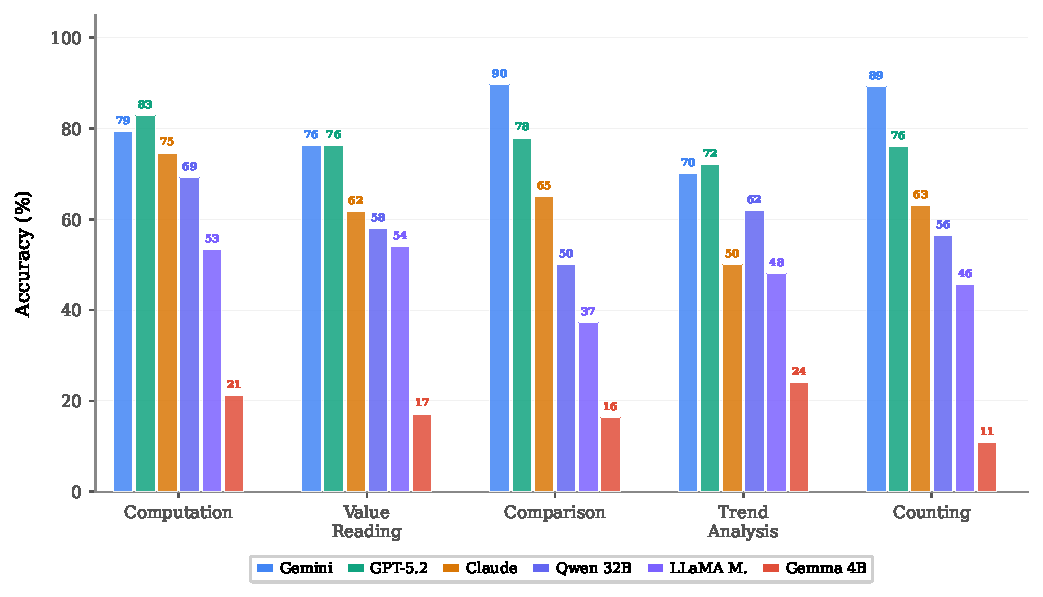
\includegraphics[width=0.80\textwidth]{figures/rq3/capability_grouped_bar.pdf}
  \vspace{-6pt}
  \caption{\textbf{Per-category capability accuracy.} Five question types on 45 figures. Comparison and counting hardest; computation easiest.}
  \label{fig:capability-bar}
\end{figure}

Four findings emerge.

First, \textbf{Gemini leads on comprehension} (.81), overtaking GPT-5.2 (.78), which led on description quality (RQ1). This suggests that description and comprehension may be partially dissociated. GPT-5.2 excels at computation (.83) but Gemini dominates comparison (.90) and counting (.89).

Second, \textbf{comparison and counting are the hardest question types} (mean .42 and .44 across models), while computation is easiest (.51). This inverts the intuition that numerical computation would be hardest; in practice, models can often compute correctly from approximate values but struggle to compare elements or count discrete visual features.

Third, \textbf{caption bias is weaker than expected}. Caption-aided accuracy (CB column) drops below baseline for several models (Qwen-235B: .36 vs .58 overall), suggesting that captions can \emph{distort} model answers by anchoring them to the caption's framing rather than the visual evidence. Proprietary models (Gemini .82, GPT-5.2 .78) resist this bias better.

Fourth, \textbf{prompt reversal resistance correlates strongly with model quality}. Gemini (.98) and GPT-5.2 (.96) are nearly immune to reversed prompts, while LLaMA Scout (.14) and Gemma-27B (.24) are highly susceptible, agreeing with whichever framing they are given. This indicates a failure of visual grounding: weaker models default to linguistic plausibility rather than image evidence.

%% ===================================================================
\section{RQ4: Behavioural Dynamics Under Stress}\label{sec:rq4-results}
%% ===================================================================

RQ4 applies our A-R-I behavioural framework to probe how models respond when visual evidence is degraded, absent, or contradicted.
We evaluate three axes: \textbf{Admittance} (epistemic honesty when content is unreadable), \textbf{Resistance} (robustness to false or unsupported premises), and \textbf{Inductance} (legitimate reasoning from partial or deceptively presented evidence).

Table~\ref{tab:ari} reports per-model scores across all three axes.
Figure~\ref{fig:ari-dotstrip} visualises the A-R-I behavioural profiles (supplementary radar and admittance breakdown in Appendix Figures~\ref{fig:app-ari-radar}--\ref{fig:app-admittance-stacked}).

\begin{table}[!ht]
\centering
\scriptsize
\setlength{\tabcolsep}{2.5pt}
\caption{\textbf{RQ4: A-R-I behavioural scores} (judge-averaged).
  Sub-component abbreviations (Pa, Ps, Ac, Ct, In, Un, I$_a$, I$_p$) are defined in Table~\ref{tab:ari-defs}.
  All scores 0--1$\uparrow$. Sorted by overall Admittance (A$\downarrow$). \textbf{Bold}/\underline{underline} = best/2nd per column.
}\label{tab:ari}
\begin{tabular}{@{}l rrr r rrr r rr@{}}
\toprule
 & \multicolumn{3}{c}{\textbf{Admittance}} & & \multicolumn{3}{c}{\textbf{Resistance}} & & \multicolumn{2}{c}{\textbf{Inductance}} \\
\cmidrule(lr){2-4}\cmidrule(lr){6-8}\cmidrule(lr){10-11}
\textbf{Model} & \textbf{Pa} & \textbf{Ps} & \textbf{Ac} & \textbf{A} & \textbf{Ct} & \textbf{In} & \textbf{Un} & \textbf{R} & \textbf{I$_a$} & \textbf{I$_p$} \\
\midrule
Gemini 3.1P    & \textbf{.55} & \textbf{.87} & \textbf{.67} & \textbf{.70} & \textbf{.96} & \textbf{.86} & \textbf{.87} & \textbf{.89} & \textbf{1.0} & .39 \\
Claude 4.6     & .51 & \underline{.57} & \underline{.27} & \underline{.45} & \underline{.67} & \underline{.66} & .74 & \underline{.69} & .80 & \underline{.50} \\
GPT-5.2        & \underline{.53} & .61 & .07 & .40 & .50 & .46 & .72 & .56 & .80 & \textbf{.89} \\
Qwen 32B       & .30 & .33 & .16 & .26 & .17 & .35 & .63 & .38 & \underline{.95} & .39 \\
Qwen 235B      & .29 & .31 & .12 & .24 & .10 & .48 & \underline{.75} & .44 & .75 & .22 \\
LLaMA Mav.     & .30 & .16 & .12 & .19 & .24 & .36 & .66 & .42 & .75 & .28 \\
LLaMA Scout    & .29 & .09 & .13 & .17 & .15 & .17 & .58 & .30 & .60 & .17 \\
Qwen 8B        & .25 & .19 & .00 & .15 & .11 & .22 & .47 & .27 & .90 & .33 \\
Phi-4          & .28 & .10 & .05 & .14 & .06 & .01 & .23 & .10 & .10 & .11 \\
Qwen 30B       & .19 & .09 & .00 & .09 & .05 & .17 & .42 & .21 & .60 & .22 \\
Gemma 27B      & .09 & .02 & .02 & .04 & .03 & .11 & .51 & .21 & .35 & .00 \\
Gemma 12B      & .05 & .03 & .00 & .03 & .06 & .14 & .52 & .24 & .30 & .00 \\
Gemma 4B       & .03 & .00 & .00 & .01 & .00 & .06 & .40 & .15 & .40 & .06 \\
\bottomrule
\end{tabular}
\end{table}

\begin{figure}[!ht]
  \centering
  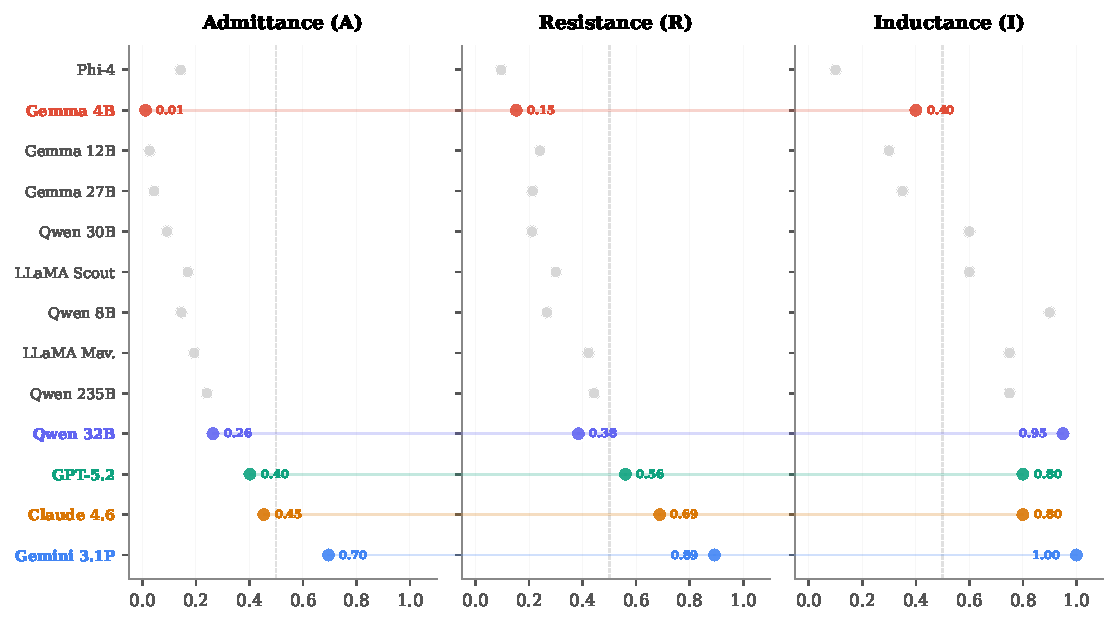
\includegraphics[width=\textwidth]{figures/rq4/ari_dotstrip.pdf}
  \caption{\textbf{A-R-I behavioural profiles} (small multiples). Each panel shows one axis; each dot is a model. Focal models (brand colours) are connected across panels by faint lines, revealing their behavioural signature. The 0.5 dashed line marks the midpoint. Gemini dominates all three axes. GPT-5.2 shows strong Inductance but weak Resistance. Gemma-4B collapses near zero on Admittance and Resistance.}
  \label{fig:ari-dotstrip}
\end{figure}

\paragraph{Admittance.}
When axis labels are blurred, models split into three response strategies: admitting uncertainty, fabricating plausible values, or remaining silent.
Gemini leads admittance (.70), admitting blurred content in 51\% of axis-blur cases and 87\% of selective-blur cases.
GPT-5.2 admits passively (.53/.61) but rarely actively (.07), suggesting it acknowledges blur implicitly through hedged language rather than explicit statements.
The Gemma family and Qwen-30B almost never admit ($\leq$.09), fabricating in $>$50\% of cases.
Claude shows a distinctive profile: moderate passive admittance (.51/.57) with the second-highest active admittance (.27), making it the most explicitly honest model after Gemini.

\paragraph{Resistance.}
Three probe types test whether models reject false premises: \emph{contra-factual} probes assert incorrect values (``the y-axis ranges from 0 to 50'' when it shows 0--100), \emph{non-existent} probes reference elements absent from the figure (``describe the dashed trend line'' when none exists), and \emph{unanswerable} probes ask questions the figure cannot answer (``is the difference statistically significant?'').
Gemini resists .89 overall, with near-perfect contra-factual resistance (.96) and strong non-existent probe rejection (.86).
GPT-5.2 is surprisingly vulnerable (.56 overall, .50 on contra-factual), often engaging with false premises rather than rejecting them.
Across all models, unanswerable questions are easiest to resist (mean .58) because models can recognise the question type, while contra-factual probes are hardest (mean .24) because they require the model to verify a specific claim against the image.

\paragraph{Inductance.}
Inductance is measured through two instruments that produce divergent rankings.
\emph{Active inductance} (I$_a$) tests reasoning on clean figures via 5 probes whose naive answer is incorrect (e.g., pie chart labels summing to 87, not 100, revealing raw counts rather than percentages).
Gemini scores 1.0 (5/5), while GPT-5.2 scores .80 (4/5).
\emph{Passive inductance} (I$_p$) tests whether models correctly infer 9 blurred elements deducible from context (Appendix Table~\ref{tab:inferable}).
Here the ranking inverts: GPT-5.2 infers 8/9 correctly (.89), while Gemini scores only .39 (judge-averaged) because it honestly admits the blur rather than attempting inference.
This dissociation illustrates the admittance--inductance tension: Gemini prioritises honesty (high A), GPT-5.2 prioritises inference (high I$_p$).
Notably, GPT-5.2 also correctly fabricates 9 of 35 \emph{non-inferable} blurred elements, raising the question of whether its inferences reflect genuine contextual reasoning or parametric recall from training data.

